\documentclass[a4paper,10pt,twoside]{paper}
\usepackage{CJK}
\usepackage{multicol}
\usepackage{graphicx}
\usepackage{subfigure}
\usepackage{booktabs}
\usepackage{amssymb,bm,mathrsfs,bbm,amscd}
\usepackage[tbtags]{amsmath}
\usepackage{lastpage}
\usepackage[justification=centering]{caption}
\usepackage{epstopdf}
\usepackage{diagbox}

\begin{CJK*}{UTF8}{gbsn}

	\begin{document}

	%\fancyhead[c]{\small Chinese Physics C~~~Vol. XX, No. X (201X)
	%XXXXXX} \fancyfoot[C]{\small 010201-\thepage}
	%\footnotetext[0]{Received XX XXXX 20XX}

	\title{Estimation of event rate and data volume in JUNO\thanks{This work is supported by the Strategic Priority Research Program of the Chinese Academy of Sciences, Grant No. XDA10010900; the CAS Center for Excellence in Particle Physics (CCEPP); National Natural Science Foundation of China (NSFC); the Chinese Academy of Sciences (CAS) Large-Scale Scientific Facility Program; Joint Large-Scale Scientific Facility Funds of the NSFC and CAS under Contracts Nos. U1332201.} }


	\author{Fang Xiao(方肖)$^{1,2}$\email{fangx@ihep.ac.cn}
		%      \quad Deng Zi-Yan(邓子艳)$^{2}$
		%     \quad Wen Liang-Jian(温良剑)$^{2}$
		%      \quad Li Wei-Dong(李卫东)$^{2}$\\
		%      \quad Yu Chun-Xu(喻纯旭)$^{1}$
		%      \quad Lin Tao(林韬)$^{2}$
	}
	\maketitle

	\address{
		$^1$ School of Physics, Sichuan University, Chengdu 610065 , China\\
		$^2$ Institute of High Energy Physics, Chinese Academy of Sciences, Beijing 100049, China\\
	}

	\begin{abstract}
		The Jiangmen Underground Neutrino Observatory (JUNO) is an experiment proposed to determine
		the neutrino mass hierarchy and probe the fundamental properties of neutrino oscillation. 
		The JUNO central detector is a spherical liquid scintillator detector with 20 kton fiducial mass. 
		The central detector's event rate is very important for JUNO online 
		electronic and DAQ(Data Acquisition)
		system design. It also help us to estimate the offline disk storage sapce for JUNO experiment data.
		So we estimate the event rate of JUNO central detector by threory and Geant4 simulation. 
		We consider many event source such
		as IBD(inverse $\beta$-decay) events, cosmic muon events, the radioactity events from materials of
		central detector, the radioactity events from water pool and rock, the PMT's dark noise events.
		We also propose and do a simulation of a promising secondary trigger system which is intend to
		suppress low energy 
		radioactity background and dark noise. The estimated disk storage sapce for JUNO experiment data
		also be gived.

	\end{abstract}


	\begin{keyword}
		JUNO, event rate, disk storage space
	\end{keyword}

	\begin{pacs}
		29.40.Mc,29.85.Fj
	\end{pacs}

	%\footnotetext[0]{\hspace*{-3mm}\raisebox{0.3ex}{$\scriptstyle\copyright$}2013
	%	Chinese Physical Society and the Institute of High Energy Physics
	%	of the Chinese Academy of Sciences and the Institute
	%of Modern Physics of the Chinese Academy of Sciences and IOP Publishing Ltd}

	\begin{multicols}{2}

		\section{Introduction}
                The Jiangmen Underground Neutrino Observatory (JUNO) is located in Kaiping, Jiangmen, in Southern China.
                It's about 53 km away from Yangjiang and Taishan nuclear power plants, both of which are under construction.
                The funding of JUNO has been approved in 2014 by China goverments, now it starts construction and expects to take data in 2020.
		JUNO\cite{lab1} is a multipurpose neutrino experiment. It is
		designed to determine neutrino mass hierarchy and precisely
		measure oscillation parameters by detecting reactor
		neutrinos from the Yangjiang and Taishan Nuclear Power
		Plants. It also intended to observe supernova neutrinos,
		study the atmospheric, solar neutrinos and geo-neutrinos,
		and perform exotic searches, more details about physics motivation can be found in Ref.yellow book. 

                Event rate and data volume of JUNO detector are essential inputs to design electronics and readout system, 
                which are used to read signals out and save them to offline disks or tapes. 
                All data taken by JUNO detector will be processed offline, so in order to reasonably estimate and prepare computing resources and storage, 
                event rate and data volume are also required.
                In this paper, event rate from different signal sources have been estimated based on JUNO detector simulation, 
                and the effects from different trigger schemes have been taken into account. Finally, the data volume is also reported.

                This paper is organized as follow: JUNO detector is introduced in section 2; signal sources are analyzed in section 3.

                However, event rate heavily depends on trigger scheme used. In JUNO, two trigger schemes are proposed, one is based on 
                JUNO detector consists of central detector and veto detector. 
                The central detector is made of 20k ton liquid scintillator contained in a 34.5 meter diameter acrylic sphere. 
                The acrylic sphere is supported by a stainless struss, on which ~17,000 PMTs are mounted. The designed energy resolution of central detector is 3\% at 1 MeV.
                The JUNO detector will be installed underground with 700 meter overburdern to suppress backgrounds from cosmic muons.
                
		Electronics, readout system and trigger are key components in JUNO.
                The experiment hall is expected to be finished at 2019. 
		It is possible to get data from the experiment at 2020.
		The JUNO central detector's event rate is very important for 
		JUNO experiment design. So we want to estimate JUNO
		event rate by theory and Geant4 simulation. The
		JUNO event rate is composed of signal rate and background
		rate.With the estimated JUNO event rate,we can estimate the necessary
		offline disk storage space for JUNO experiment data and help the 
		online electronic and DAQ system design.
		
		We also propose and do a simulation of a promising secondary trigger system which is intend to
		reduce the event rate of low energy 
		radioactity background and dark noise. 

		In the beginning, for the central detector we proposed
		three design options: acrylic option, balloon option and 
		module option. According to the Geant4 detector simulation,
		the module option was abandoned. Since the acrylic option
		and balloon option are similar, we study the acrylic option
		to estimate the event rate of JUNO central detector.


		%For the backgrounds such as natural radioactivity background(U, Th, K), cosmic muons, the event rate of JUNO is possibly large.  


		\section{JUNO detector}
		The JUNO detector is composed of a central detector, a water
		cherenkov detector and a muon tracker(shown in Fig.1). The 
		central detector is made of 20k ton liquid scintillator contained in a 34.5 meter diameter acrylic sphere.
                The acrylic sphere is supported by a stainless-steel truss, on which 17,000 PMTs are mounted to detect scintillation lights from LS. 
		CD(Central Detector) will be installed in a water pool used to shield background of natural radioactivities from surrounding rock and environment. 
                The water pool is also a water cherenkov detector which can tag cosmic muons by detecting cherenkov lights. 
                Water between PMT and acrylic sphere can also be used as a buffer to shield radioactivity background from PMTs and stainless-steel truss.
                The thickness of the buffer is about 1.4 meter. On the top of CD, a muon tracker will be intalled to detect muons with better position and direction resolution.
                The designed energy resolution of CD can reach 3\% at 1 MeV, corresponding to 1100 pe/MeV of energy scale.

                Electronics and readout system need to cope with signals from 17,000 PMTs when an event is triggered.
                Several electronics schemes have been proposed, depending on where to put electronics units.
                FADC is proposed to digitize the signal of a fired PMT with 1GHz sampling rate.
                All data from FADC are transmitted to online computing farm through data links.

                Trigger system is essential for JUNO detector, which is used to reject backgrounds as much as possible and keep high detection efficiency for physical events.
                A common trigger strategy is to tag events using multiplicity of fired PMTs, which has been successfully used in Daya Bay experiment. It can reach 100\% trigger
                efficiency for IBD events with 0.5 MeV trigger threshold. However, for some scientific motivations, like solar neutrino and supernova neutrino, a much lower 
                trigger threshold is preferred. But the lower trigger threshold is limited by coincidence of PMT dark noise. 
                So a sophisticated trigger method is proposed based on vertex fitting, it will be discussed more in next section.
                
		\begin{center}
			%\includegraphics[width=6cm]{acrylicoption.png}
			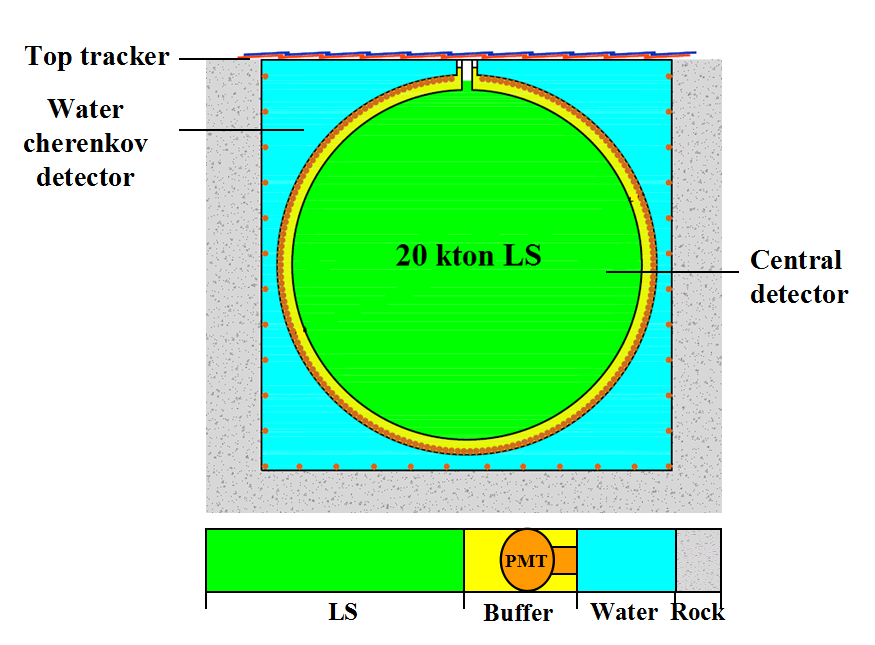
\includegraphics[width=7cm]{CD.png}
			\figcaption{\label{fig2}   Schematic view of the JUNO detector}
		\end{center}


		\section{Events rate of physical events in CD}

		%In JUNO experiment, particles deposit energy in LS and release
		%photons.If the energy of the photons which detected by the PMT
		%exceed the trigger system's energy threshold, the detector will
		%record the electronic output information as a event.
                When particles deposit their energy in LS, LS can be excited and emits scintillation lights during deexcitation.
                The amount of scintillation lights is proportional to the quenched deposited energy, in which quenching effects are considered.
                Different particles have the different quenching factors. The scintillation lights and Cherenkov lights, if particle's velocity is larger than light velocity in LS, can be detected by PMTs in CD,
                then converted to photo-electrons and PMT pulses after processing electronics system. Finally, if the amount of light is enough to fire a trigger, readout system will save PMT signals within a readout time window and form an event.

                
		The events detected by CD can be divided into physical events and background events. Physical events include all events that we are interested in, 
                like reactor neutrino, solar neutrino, geo-neutrino, atmesphere neutrino, etc.
                For each physical channel, the original event rate has been well 
                estimated in JUNO yellow book. Combining its energy spectrum, 
                the event rates of each physics with different threshold of multiplicity trigger are summarized in table 1.

        \begin{center}
                \tabcaption{ \label{tab1}  rates of different event source} 
                \footnotesize
                \begin{tabular*}{80mm}{@{\extracolsep{\fill}} c c }
			\toprule  event source&Rates  \\
                        \hline
                        IBD event               & 83 per day   \\
                        Li9/He8 $\beta$-n decay & 84 per day   \\
                        fast neutron            & 0.1 per day  \\
                        C13($\alpha$,n)O16      & 0.05per day  \\
                        Geo-neutrino            & 1.5 per day  \\
                        cosmic muon             & 3Hz          \\
                        Natural Radioactivity   & 1006702.8Hz  \\
			Solar neutrino          & 0.45Hz       \\
			Atmospheric neutrino    & 0.94per day  \\
                        \bottomrule
                \end{tabular*}
        \end{center}

                
                The solar neutrino is a major source to events rate of physical events, which can reach 0.45 Hz totally if no trigger threshold is applied, and is mainly from pp channel.
                But, the energy of pp neutrino is quite low. If only a simple multiplicity trigger is chosen, the trigger threshold can not be lower than 0.5 MeV 
                due to limitation of radioactivity background and coincidence of PMT dark noise. With 0.5 MeV threshold, most of pp neutrino will be discarded by trigger system, the solar neutrino events rate becomes 0.04 Hz.

                The total events rate from physical channel is less than 1 Hz, which is negligible comparing with that from radioactivity background.
                However, if a supernova bursts at a typical distance of 10kpc, neutrino events rate has been estimated to be hundreds of Hz from different channels, 
                and events rate is much higher in the first second during explosion. The supernova can sustain for about 10 seconds. 
                In JUNO, all data in 10 seconds will be read out without trigger threshold. For a supernova with shorter distance, the higher events rate is expected. 
                
                
                \section{Events rate of background events in CD}
                \subsection{Radioactivity background}
                One of main contributions to event rate is natural radioactivity background, which comes from various sources, like $^{238}$U, $^{232}$Th ,$^{40}$K. 
                They come from different materials in JUNO detector. In order to control the event rates of background, the purity of each material used to make detector is required by mass hierachy sensitivity.
		In Daya Bay experiment, the U/Th concentrates in LS are 4$\times10^{-5}$ g/g and 2$\times10^{-5}$ g/g respectively.
		In JUNO, a better purification system will be applied, which can reduce the U/Th two order of magnitude, to the level of $10^{-6}$ g/g. For $^{40}$K, it can reach $10^{-7}$ g/g. 
		Besides U/Th/K, cosmic muons continuously produce $^{14}$C from $^{14}$N, via the reaction $^{14}$N(n,p)$^{14}$C.
		If the petroleum used to make LS are located deep underground and are shielded from high cosmic ray flux, one can expect very low $^{14}$C contanimation in LS. 
		But for worst case, petroleum may locate on the surface of earth which suffer with very high flux of cosmic muons, $^{14}$C abundance is esimated to be $10^{-18}$ g/g.
		The radioactivity in PMT glass depends on which glasses are selected to make PMTs.
		In this paper, the shott glass is used for event rate studes and its U/Th/K concentrations are 22ppb, 20ppb and 3.54ppb respectively.
		For other glasses, the impacts can be easily scaled based on results of shott glass. 
		However, due to 1.4 meter water buffer between PMTs and LS, the event rate from PMT glass can be reduced a lot. This effect has been included in our simulation.
                The acrylic sphere is quite closed to LS in which the radioactivity can easily deposit their energies in LS and be triggered to form events.
                Radioactivity existing in stainless truss also contributes total events rate in CD, but silimar with that in PMT glass, it is heavily suppressed by water buffer.
                U/Th/K concentration in stainless truss are proposed to be 1.2 mBq/kg, 8.0 mBq/kg and 13.4 mBq/kg respectively based on Ref.XinYing.
		$^{60}$Co can also be generated when cosmic muons go through stainless truss.
                Many copper plates are used to support acrylic shpere, and radioactivity in copper has to be taken into account in event rate studies.
		The contamination in copper depends on technology to make high purity copper. Based on experiences from Ref., 1.23 mBq/kg $^{238}$U, 0.405 mBq/kg $^{232}$Th and 0.0377 mBq/kg $^{40}$K in copper are used in this study. 
		Fast neutrons produced by cosmic muons reacting on $^{63}$Cu produce $^{60}$Co. $^{60}$Co abundance is 0.3 mBq/kg.
                Radon in water is requied to be less than 0.2 Bq/m3, then no significant effects on MH senstivity. And U/Th/K concentrations in rock are 10ppm, 30ppm and 5ppm respectively.
                The radioacitivity impurity in different materials are summarized in table 2. 

	\end{multicols}
	\begin{center}
		\tabcaption{ \label{tab1}  The proposed concentration of radioactive impurity in different detector materials.}
		\footnotesize
		\begin{tabular*}{190mm}{@{\extracolsep{\fill}}ccccccccc}
			\toprule \hphantom{0} & $^{238}$U & $^{232}$Th & $^{40}$K  & $^{210}$Pb & $^{85}$Kr & $^{39}$Ar & $^{60}$Co & $^{14}$C\\
			\hline
			LS & $10^{-6}$ ppb & $10^{-6}$ ppb & $10^{-7}$ ppb & $1.4\cdot10^{-13}$ ppb & 50 $\mu Bq/m^3$ & 50 $\mu Bq/m^3$ & \~{}  & 1$\times10^{-18}$g/g \\
			Glass & $22$ ppb & $20$ ppb & $3.54$ ppb & \~{} & \~{} & \~{} & \~{} & \~{} \\
			Acrylic & $10$ ppt  & $10$ ppt & $10$ ppt & \~{} & \~{} & \~{} & \~{} & \~{} \\
			Steel & $ 1.2$ mBq/kg & $8.0$ mBq/kg  & $13.4$ mBq/kg & \~{} & \~{} & \~{}& $2.0 $ mBq/kg  & \~{} \\
			Copper & $1.23$ mBq/kg  & $0.405$ mBq/kg & $0.0377$ mBq/kg & \~{} & \~{} & \~{} & $0.3 $ mBq/kg & \~{} \\
			\bottomrule
		\end{tabular*}
	\end{center}

	\begin{multicols}{2}


		A detailed detector simulation software has been implemented based on Geant4. For each material in JUNO detector, 
		the radioactivity listed in table 2 are used in detector simulation to study its events rate.
		The results with different trigger thresholds are summarized in table 3, the multiplicity trigger is used as default.

	\end{multicols}
	\begin{center}
		\tabcaption{ \label{tab1}  The inner singles rates} 
		\footnotesize
		\begin{tabular*}{170mm}{@{\extracolsep{\fill}} c c c c c c c c c}
			\toprule  Singles Rate(Hz)&LS &Glass &Acrylic  &Steel &Copper &Rn &Rock  &Sum \\
			\hline
			E$>$0.7MeV &2.39   &2.43  &69.23  &0.89  &0.82 &15.94 &7.42     &99.12   \\
			E$>$0.6MeV &4.26   &2.66  &75.26  &0.95  &0.94 &19.79 &8.1223   &111.982 \\
			E$>$0.5MeV &12.06  &2.83  &81.49  &0.98  &1.06 &23.36 &8.6414   &130.421 \\
			E$>$0.4MeV &13.86  &3.24  &87.84  &1.22  &1.29 &26.11 &9.89333  &143.453 \\
			E$>$0.3MeV &15.51  &3.72  &98.57  &1.57  &1.51 &31.60 &11.359   &163.839 \\
			E$>$0.2MeV &17.16  &4.12  &117.33 &1.80  &1.89 &39.85 &12.5804  &194.73  \\
			E$>$0.1MeV &352.36 &5.27  &149.26 &2.22  &2.60 &54.97 &16.0919  &582.772 \\
			\bottomrule
		\end{tabular*}
	\end{center}
	\begin{multicols}{2}


		The events rate increases when the trigger threshold discreases. For a normal threshold of 0.5 MeV, the total events rate is about 130 Hz.
		Acrylic and Radon in water are two major sources of events. For radioactivity in LS, the events rate is suddenly changed from 17 Hz to 352 Hz.
		It is caused by $^{14}$C in LS generated by cosmic muons. $^{14}$C goes through radioactive beta decay by emitting an electron and an electron antineutrino.
		The emitted electrons have a maximum energy of 0.156 MeV and can not be triggered with 0.2 MeV threshold. 
		While, a fraction of $^{14}$C can be triggered by 0.1 MeV threshold.

		\subsection{Cosmic muons}
		JUNO detector is located uderground with 748m overburder. By considering the detailed map at JUNO site, the cosmic ray flux can be simulated by MUSIC.
		Then, the muon flux in experimental hall is obtained to be 0.003Hz/m2, and the average energy of muons are determined to be about 215 GeV.
		Based on muon flux and dimensions of CD, the total muon events rate in CD is calculated to be 3 Hz.

		The cosmic muons which go into the CD can be seperated into shower muons and non-shower muons. The non-shower muons are minimal ionization particles.
		The shower muons may generate neutrons and radioactivity isotopes with long lifetime, 
		which can form delayed signals and be tagged as seperated events besides muon track itself. 20\% of muons are shower muons from simulation.
		And after processing a detailed muon simulation, we found that the events rate induced by muons is about 5 Hz totally.


		\subsection{PMT dark noise}
		Coincidence of PMT dark noise also has probabilities to trigger an event, depending on trigger threshold.
		In JUNO, since ~17,000 20 inch PMTs will be installed, it is much easier to be coincident in a readout time window and trigger an event, 
		comparing with that in Daya Bay experiment, in which only 192 8 inch PMTs are used in each anti-neutrino detector.
		While the probability of PMT dark noise coincidence can be accurately calculated using the formula:

		\begin{displaymath}
			R = \frac{1}{\tau}\sum_{i=m}^{N}iC^{i}_{N}(f\tau)^i
			(1-f\tau)^{N-i}
		\end{displaymath}

		in which, N is the number of PMTs and m is number of fired PMTs that determined by trigger threshold, assuming multiplicity trigger is used.
		f denotes dark rate of each PMT; $\tau$ indicates length of trigger time window.

		The total PMT number is assumed to be 17746 during calculation of coincident probability. 
		And MCP-PMTs are assumed to use in JUNO detector. The dark rate of each MCP-PMT is 50kHz. 300ns of trigger time window is selected.
		The calculated events rate versus trigger threshold is shown in Fig 2, in which the re-trigger is allowed,
		and assuming single photo-electron on each fired PMT caused by dark noise.
		The numbers of fired PMTs are also converted into energy based on energy scale of 1100pe/MeV.

		\begin{center}
			%\includegraphics[width=6cm]{acrylicoption.png}
			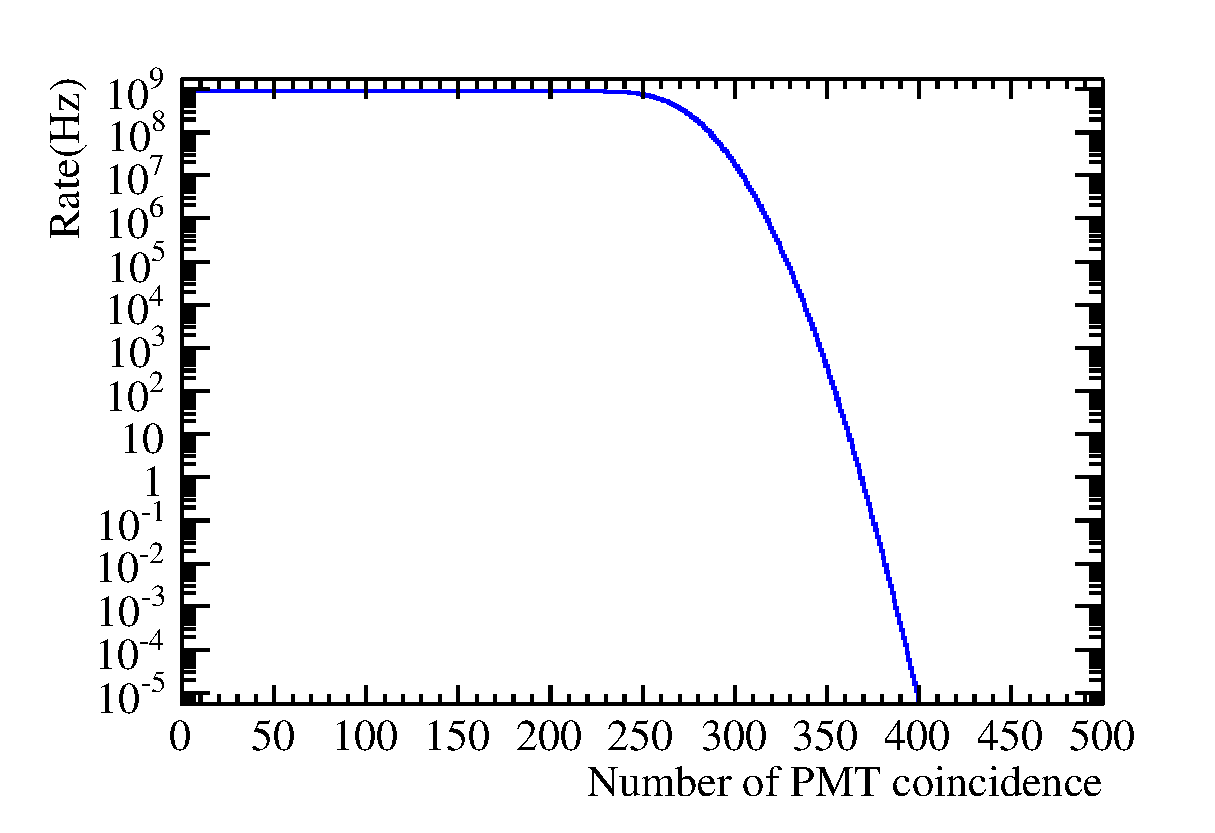
\includegraphics[width=8cm,height=6cm]{Noise_rate_50kHz_300ns.eps}
			\figcaption{\label{fig2}
				Dark noise event rate when trigger integration time is 300ns
			}
		\end{center}


		In order to suppress events from coincidence of dark noise, the trigger threshold should be greater than 0.5MeV, 
		and the corresponding events rate can be negligible. Although the lower trigger threshold is preferred by some physics topics,
		it is not achievable by simple multiplicity trigger limitted by PMT dark noise. A sophisticated trigger method will
		be discussed in next section, which allows lower trigger threshold. 


		\subsection{A sophisticated trigger scheme}

		The multiplicity trigger with 0.5 MeV trigger threshold is good enough for mass hierarchy measurements and most of other physics. 
		But the lower trigger threshold is also preferred by solar neutrinos and supernova neutrinos.
		Since the threshold of multiplicity trigger is limited by PMT dark noise, a sophisticated trigger scheme is proposed.
		Events can be triggered by either of these two trigger schemes. A simple idea is to shorten trigger time window to reduce effects from dark noise.
		If events positions are known for trigger system, time of flight (TOF) of light can be corrected, and then a shorter trigger window can be used.
		But, in other hands, events from radioactivity will increase when trigger threshold decreases.
		Because most of radioactivity are from outer region of CD, a fiducial volume cut should be very effective to reduce events rate of radioactivity.
		FPGA can not handle complex position reconstruction algorithms, so a simple method is used to reconstrut event position with acceptable position resolution.
		Using this method, CD is divided into 179 cubic volumes. For each volume, the dimension is 5m$\times$5m$\times$5m.
		To get the event position, the time of flight in each volume is corrected for each PMT. If a volume contains the event, 
		the narrowest the first hit time distribution on all fired PMTs should be gotten. 
		Then, the center of this cubic volume is taken as the event position.
		This method has been proved and validated by simulations, and events rate with this new trigger scheme are also studied.

		Fig.3 and Fig. 4 show the first hit time distribution on PMTs in the volume containning an event without and with TOF correction, 
		by simulating 4MeV e+ at (15,0,0) in CD. After applying TOF correction, a much narrower distribution is obtained.
		For other volumes, which don't contain the generated position of event, hit time distribution is broader, shown in Fig. 5 as an example.
		Based on the first hit time distribution after TOF correction, a multiplicity trigger is applied again, but trigger time window can be reduced from
		300ns to 50ns. 

		\begin{center}
			%\includegraphics[width=6cm]{acrylicoption.png}
			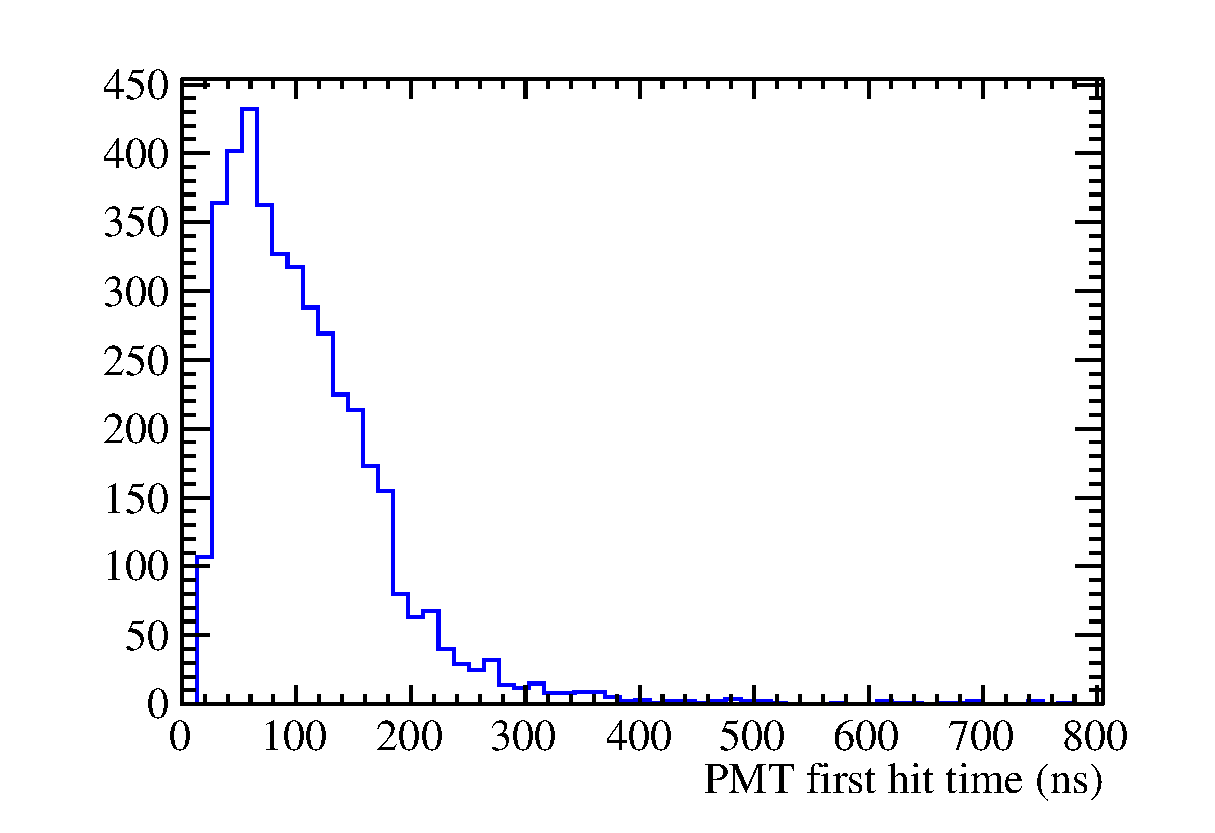
\includegraphics[width=8cm,height=6cm]{4MeV_e+_PMT_first_hitTime.eps}
			\figcaption{\label{fig2}   PMT's first hit time without TOF corrected 
			}
		\end{center}


		\begin{center}
			%\includegraphics[width=6cm]{acrylicoption.png}
			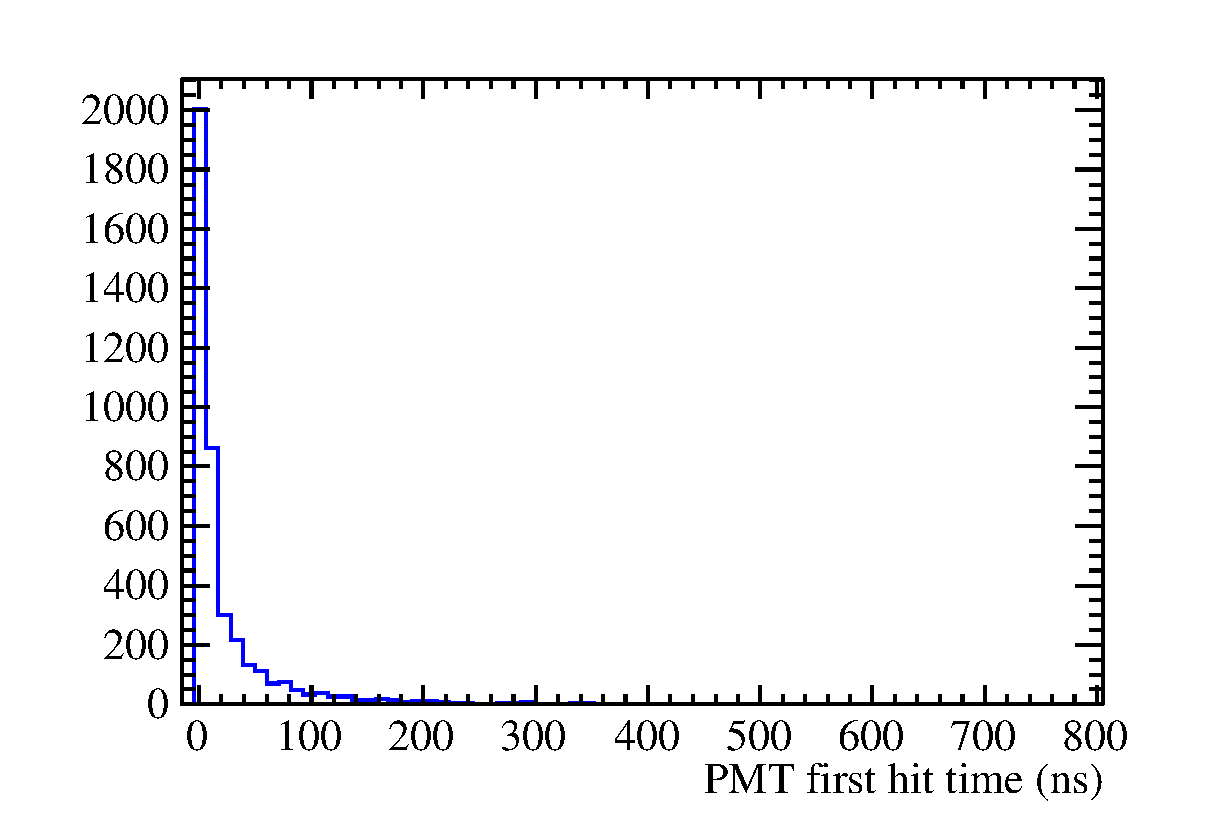
\includegraphics[width=8cm,height=6cm]{4MeV_e+_PMT_first_hitTime_corrected.eps}
			\figcaption{\label{fig2}   PMT's first hit time with TOF corrected 
			}
		\end{center}


		The reconstructed positions are also validated by using the truth positions gotten from Monte Carlo (MC) truth information. 
		The bias between reconstructed and truth event positions are drawn in Fig. 6, by using 14C events in LS. 

		\begin{center}
			%\includegraphics[width=6cm]{acrylicoption.png}
			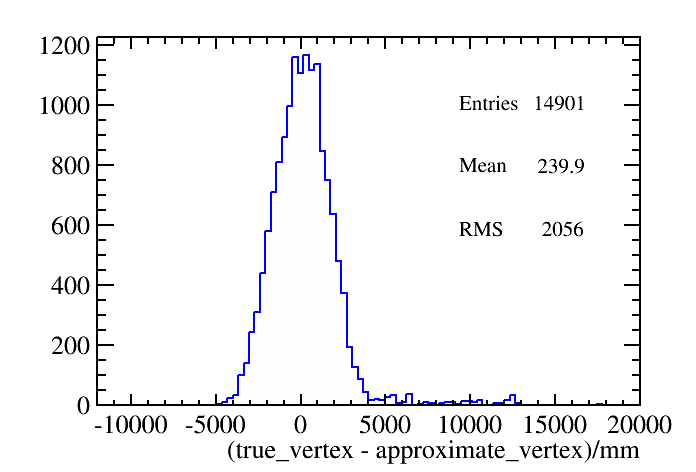
\includegraphics[width=7cm]{C14_deltaR.png}
			\figcaption{\label{fig2}   Delta of true C14 event vertex and reconstructed approximate event vertex}
		\end{center}

		The largest bias in Fig. 6 is smaller than the volume size, 5 meter, which means the volume can be 100\% correctly found.
		The resolution of reconstructed positions is about 1.55 meter, which agrees with expections.


		To take the numbers in table 1 as the inputs of simulations, events rate from background are estimated again with new trigger scheme. 
		The events rate from different radioactivity sources are summed up and the results are listed in table 2 with different trigger threshold and in
		different fiducial volumes.


	\end{multicols}
	\begin{center}
		\tabcaption{ \label{tab1} The sum radioactivity singles rates in central detector on different energy and radius threshold }
		\footnotesize
		\begin{tabular*}{170mm}{@{\extracolsep{\fill}} c c c c c c c}
			\toprule  Sum Radioactivity Single Rate(Hz)&E$>$0.1MeV & E$>$0.2MeV & E$>$0.3MeV & E$>$0.4MeV & E$>$0.5MeV & E$>$0.6MeV \\
			\hline
			%rate with out rock rateR$<$10m &142.368  &98.332  &96.9047 &95.9515 &95.2811  &93.7126 \\
			%			R$<$11m &153.808  &99.1398 &97.5285 &96.4432 &95.6678  &93.8127 \\
			%			R$<$12m &199.79   &102.354 &100.039 &98.4438 &97.2644  &94.2101 \\
			%			R$<$13m &249.897  &105.33  &102.395 &100.341 &98.7855  &94.5798 \\
			%			R$<$14m &249.897  &105.33  &102.395 &100.341 &98.7855  &94.5798 \\
			%			R$<$15m &289.921  &112.385 &107.156 &103.627 &101.128  &95.4422 \\
			%			R$<$16m &458.269  &148.923 &131.168 &119.73  &112.381  &99.866  \\
			%			R$<$17m &540.865  &173.071 &146.688 &129.847 &119.277  &102.776 \\
			R$<$10m &146.299  &104.685  &103.623  &102.569  &101.594  &100.510  \\  
			R$<$11m &158.055  &105.545  &104.290  &103.094  &102.007  &100.617  \\
			R$<$12m &205.307  &108.967  &106.975  &105.233  &103.709  &101.043  \\
			R$<$13m &256.797  &112.135  &109.494  &107.261  &105.331  &101.440  \\
			R$<$14m &256.797  &112.135  &109.494  &107.261  &105.331  &101.440  \\
			R$<$15m &297.926  &119.646  &114.585  &110.774  &107.829  &102.365  \\
			R$<$16m &470.923  &158.544  &140.262  &127.987  &119.827  &107.109  \\
			R$<$17m &555.812  &184.252  &156.858  &138.802  &127.180  &110.231  \\

			\bottomrule
		\end{tabular*}
	\end{center}
	\begin{multicols}{2}

		Events rate caused by PMT dark noise coincidence is re-calculated with 50ns trigger time window, 
		using the similar method discussed in previous sections. The calculated events rates are shown in Fig. ??.
		Using the new trigger scheme, trigger threshold can be reduced to 0.2 MeV, and events rate from radioactivity is still under control.

		\begin{center}
			%\includegraphics[width=6cm]{acrylicoption.png}
			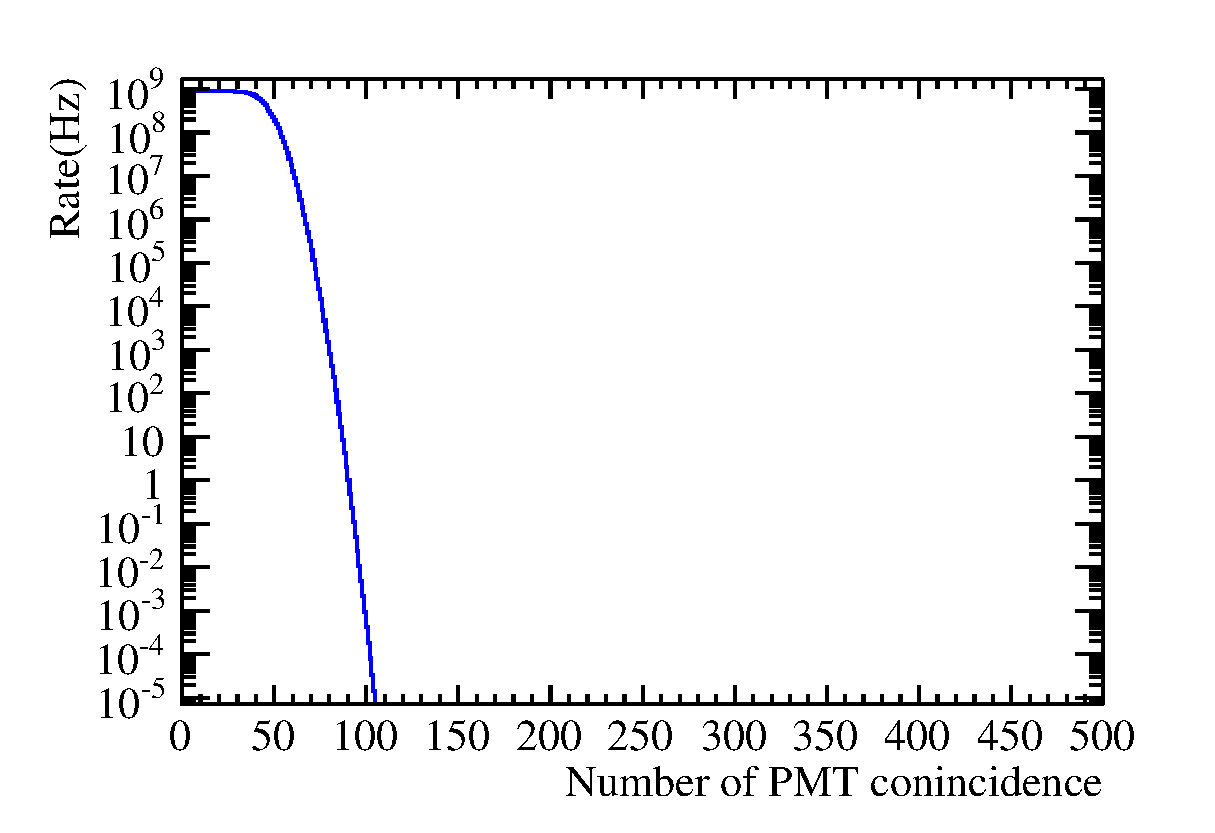
\includegraphics[width=8cm,height=6cm]{Noise_rate_50kHz_50ns.eps}
			\figcaption{\label{fig2}
				Dark noise event rate when trigger integration time is 50ns
			}
		\end{center}

		\section{Estimation of data volume in JUNO}
		JUNO is proposed to run at least 6 years for neutrino mass hiarachy measurements and other physics topics. 
		It's important for offline data processing and disk storage preparation to estimate the data volume after 6 years running. 
		Different events have different event size, depending on number of photo-electrons detected by CD.
		Fig. ?? shows the PE numbers from different event sources, including radioactivity events and different physical events. 



	\end{multicols}
	\begin{center}
		\tabcaption{ \label{tab1} The DAQ data rate of central detector on different energy and radius threshold }
		\footnotesize
		\begin{tabular*}{170mm}{@{\extracolsep{\fill}} c c c c c c c}
			\toprule  DAQ data rate(MBytes/s)&E$>$0.1MeV & E$>$0.2MeV & E$>$0.3MeV & E$>$0.4MeV & E$>$0.5MeV & E$>$0.6MeV \\
			\hline
			R$<$10m &400.598  &317.369  &315.246  &313.138  &311.188  &309.020  \\  
			R$<$11m &424.110  &319.089  &316.580  &314.189  &312.013  &309.234  \\
			R$<$12m &518.613  &325.933  &321.949  &318.466  &315.418  &310.087  \\
			R$<$13m &621.595  &332.270  &326.988  &322.522  &318.662  &310.880  \\
			R$<$14m &621.595  &332.270  &326.988  &322.522  &318.662  &310.880  \\
			R$<$15m &703.853  &347.291  &337.170  &329.547  &323.657  &312.730  \\
			R$<$16m &1049.85  &425.088  &388.524  &363.975  &347.654  &322.219  \\
			R$<$17m &1219.60  &476.504  &421.716  &385.604  &362.360  &328.461  \\

			\bottomrule
		\end{tabular*}
	\end{center}
	\begin{multicols}{2}


		If electronic system can't do waveform compression, we need do waveform compression in DAQ system and
		then save the data to disk. With the waveform compression for low energy events, we can 
		shorten the waveform  length from
		1 $\mu$s to 50ns. So each low energy event contributes 0.1MBytes data, the estimated disk storage
		space is listed in table.4.

	\end{multicols}
	\begin{center}
		\tabcaption{ \label{tab1} The disk storage space of central detector on different energy and radius threshold }
		\footnotesize
		\begin{tabular*}{170mm}{@{\extracolsep{\fill}} c c c c c c c}
			\toprule  disk storage space(MBytes/s)&E$>$0.1MeV & E$>$0.2MeV & E$>$0.3MeV & E$>$0.4MeV & E$>$0.5MeV & E$>$0.6MeV \\
			\hline
			R$<$10m  &122.630  &118.468  &118.362  &118.257  &118.159  &118.051 \\  
			R$<$11m  &123.806  &118.554  &118.429  &118.309  &118.201  &118.062 \\
			R$<$12m  &128.531  &118.897  &118.697  &118.523  &118.371  &118.104 \\
			R$<$13m  &133.680  &119.213  &118.949  &118.726  &118.533  &118.144 \\
			R$<$14m  &133.680  &119.213  &118.949  &118.726  &118.533  &118.144 \\
			R$<$15m  &137.793  &119.965  &119.459  &119.077  &118.783  &118.236 \\
			R$<$16m  &155.092  &123.854  &122.026  &120.799  &119.983  &118.711 \\
			R$<$17m  &163.580  &126.425  &123.686  &121.880  &120.718  &119.023 \\

			\bottomrule
		\end{tabular*}
	\end{center}
	\begin{multicols}{2}




		\section{Conclusion}
		\vspace{-1mm}
		\centerline{\rule{80mm}{0.1pt}}
		\vspace{2mm}

		\begin{thebibliography}{90}

				\vspace{3mm}

			\bibitem{lab1}Y.F. Li, J. Cao, Y.F. Wang and L. Zhan. Unambiguous Determination of the Neutrino Mass Hierarchy Using Reactor Neutrinos. Phys. Rev. D 88, 013008 (2013).
			\bibitem{lab2}KamLAND Collaboration, K. Eguchi et al. Phys. Rev. Lett.90, 021802 (2003), hep-ex/0212021.
			\bibitem{lab3}CHOOZ Collaboration, M. Apollonio et al. Eur. Phys. J. C27, 331 (2003), hep-ex/0301017.
			\bibitem{lab4}Borexino Collaboration, C. Arpesella et al. Phys. Lett. B658, 101 (2008), astro-ph/0708.2251.
			\bibitem{lab5}Daya Bay Collaboration, F.P. An et al. Observation of electron-antineutrino disappearance at Daya Bay, Phys. Rev. Lett. 108, 171803 (2012).
			\bibitem{lab6}Double Chooz Collaboration, Y. Abe et al. Indication for the disappearance of reactor electron antineutrinos in the Double Chooz experiment, Phys. Rev. Lett. 108, 131801 (2012).
			\bibitem{lab7}Soo-Bong Kim et al. Observation of Reactor Electron Antineutrino Disappearance in the RENO Experiment, Phys. Rev. Lett. 108 (2012) 191802
			\bibitem{lab8}Soo-Bong Kim et al.  of Reactor Electron Antineutrino Disappearance in the RENO Experiment, Phys. Rev. Lett. 108 (2012) 191802
			\bibitem{lab9}Soo-Bong Kim et . Observation of Reactor Electron Antineutrino Disappearance in the RENO Experiment, Phys. Rev. Lett. 108 (2012) 191802
			\bibitem{lab10}Soo-Bong Kim . Observation of Reactor Electron Antineutrino Disappearance in the RENO Experiment, Phys. Rev. Lett. 108 (2012) 191802
			\bibitem{lab11}et al. Observation of Reactor Electron Antineutrino Disappearance in the RENO Experiment, Phys. Rev. Lett. 108 (2012) 191802



		\end{thebibliography}

	\end{multicols}

	%\clearpage
\end{CJK*}
\end{document}
